\section{Background}
\label{background}

The World-Wide Web (WWW), commonly known as the web, was invented to allow remote collaborators to share information and ''to be a pool of human knowledge'' \parencite[76]{BernersLeeCailliauLuotonenNielsenSecret1994}. HyperText Markup Language (HTML), Cascading Style Sheets (CSS), and JavaScript (JS) are considered the core web technologies \parencite{MajchrzakBiornHansenGronli2018}. The core web technologies that are all being used today were all introduced in just a few years in 1993 to 1996 (Figure \ref{webtechnologies-timeline}).

\begin{figure}[!h]
\centering
%\fbox{
    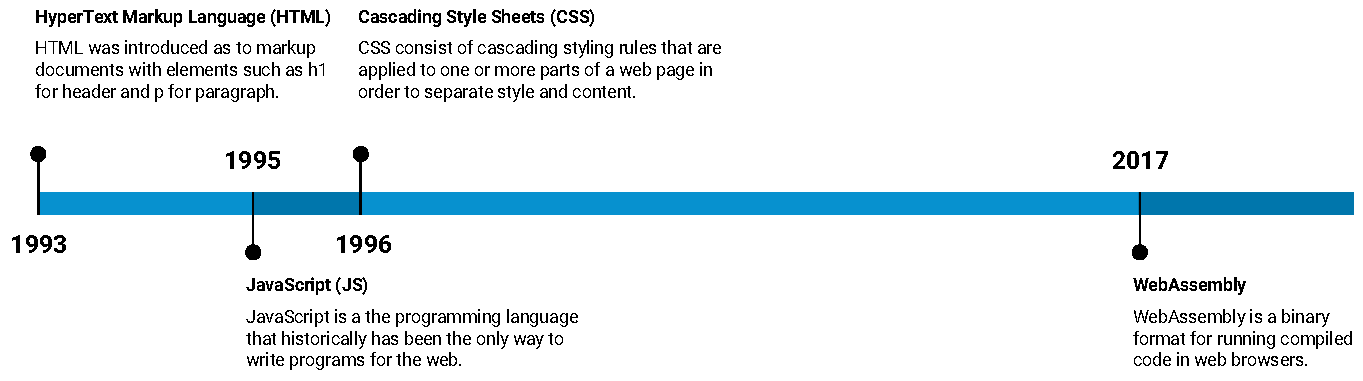
\includegraphics[width=16cm,keepaspectratio]{figures/webtechnologies-timeline}
%}
\caption{Timeline of major web technologies: HTML, CSS, JavaScript and the newest member WebAssembly.}
\label{webtechnologies-timeline}
\end{figure}

The very first web page (Figure \ref{world-wide-web}) was written in HTML and relies heavily on hyperlinks \parencite{BernersLeeCailliauGroffPollermann1992}. In 1996 the W3C recommendation on CSS was published \parencite{LieBos1996}, as a simple mechanism that ''allows authors and readers to attach style (e.g. fonts, colors and spacing) to HTML documents'' \parencite*[1]{LieBos1996} based on CSS rules. JavaScript was introduced in 1995 and was only intended to be used for simple tasks such as client-side form validation or simple animations \parencite{Moller2018}. The capabilities of JavaScript evolved and led to inventions such as Asynchronous JavaScript and XML (AJAX) \parencite{NielsonWilliamsonArlitt2008} and heavy manipulation of the Document Object Model (DOM) \parencite{WoodLeHorsApparaoByrneChampionIsaacsJacobsNicolRobieSutor1998}.

\begin{figure}[!h]
\centering
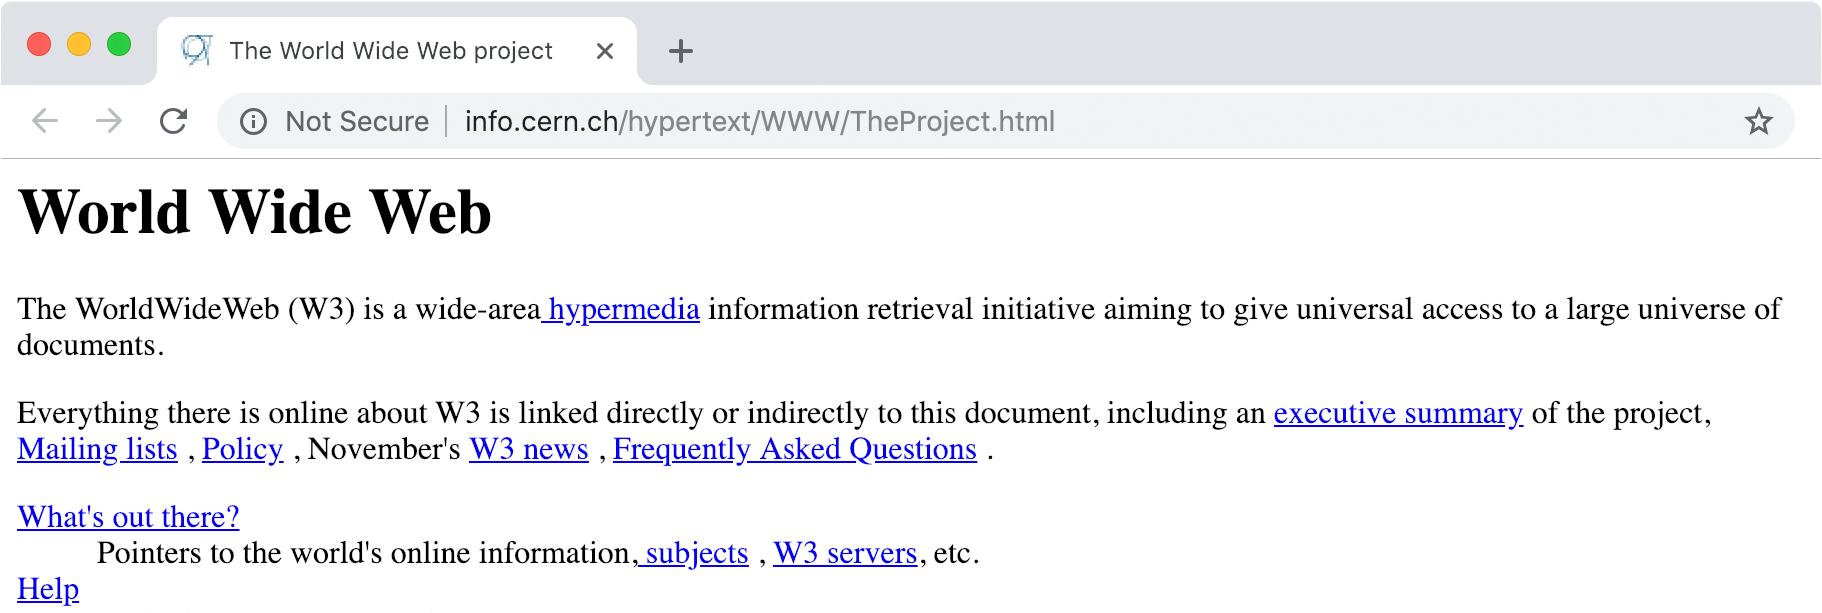
\includegraphics[width=16cm,keepaspectratio]{figures/world-wide-web}
\caption{The first web page created by Tim Berners-Lee.}
\label{world-wide-web}
\end{figure}

The introduction and evolution of JavaScript has lead the evolution of the web browser as a web page reader towards a platform for web applications.

\subsection{Web apps}

JavaScript was an important addition to the set of web technologies as it is the foundation for web applications \parencite{ParkJungMoon2015}. Since the introduction, evolution and increased performance of JavaScript, the web has evolved from simply being a platform for websites to also be a platform for web applications \parencite{SandhuHerreraHendren2018}. Web applications, or web apps for short, is a type of application that run inside a web browser. Web apps require no installation and runs on any computing device for which there is a web browser \parencite{RatanaworabhanLivshitsZorn2010}. Figure \ref{google-docs} illustrates Google Docs, a complete word processing application for the web.

\begin{figure}[!h]
\centering
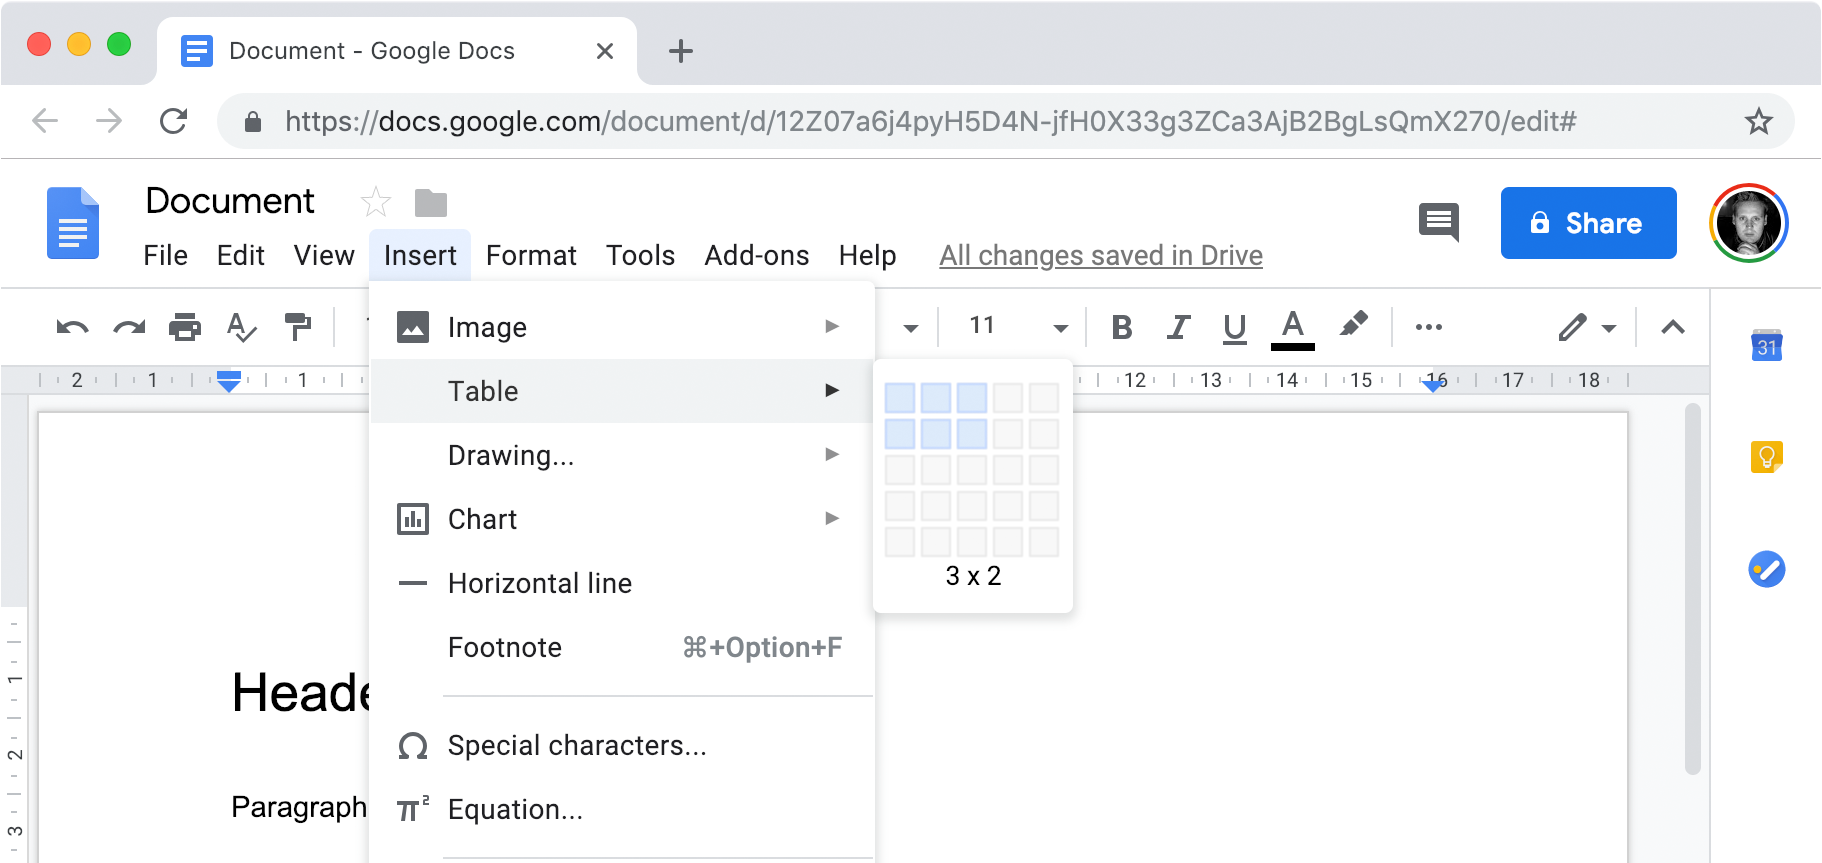
\includegraphics[width=16cm,keepaspectratio]{figures/google-docs}
\caption{Google Docs is a modern web application that enables users to do word processing in a web browser.}
\label{google-docs}
\end{figure}

Traditionally web applications was built with a thin user interface layer through which the user interacted with the application, while the actual computation was executed on one or more servers, % in the cloud
passing data back and forth between the client and the server. As modern devices becomes increasingly more powerful, more and more web apps are built to do computing client side.

\textcite{SandhuHerreraHendren2018} describe JavaScript as increasingly popular for building high performance apps and \textcite{RatanaworabhanLivshitsZorn2010} describes the complexity of web apps as the catalyst for browser vendors to increase JavaScript performance. According to \textcite{RatanaworabhanLivshitsZorn2010} the increased usage of sophisticated mobile phones also increasing the importance of web apps.

\subsection{JavaScript}

JavaScript is well supported in virtually all web browsers on both desktop and mobile \parencite{Zakai2011}. According to \textcite{TiwariSolihin2012} more than 95\% of all web pages are viewed with JavaScript enabled web browsers and more than 99\% of all web sites use JavaScript. However, while web apps have an advantage of portability compared to native mobile apps, the dynamic typing and prototypes features of JavaScript makes it execution inefficient \parencite{ParkJungMoon2015}. \textcite{HaasRossbergSchuffTitzerHolmanGohmanWagnerZakaiBastien2017} notes that while the web has given rise to demanding web apps, JavaScript as a language being the only programming language available in web browsers, is not very well equipped to support such applications. \textcite{ReiserBlaser2017} describe that there is always a desire for higher performance in web applications and \textcite{Zakai2018} describe JavaScript as an obstacle for demanding high-performing apps. The last few years manufacturers of web browsers has been focused on optimizing JavaScript performance through just-in-time (JIT) and ahead-of-time (AOT) compilation \parencite{HerreraChenLavoieHendren2018}.

\begin{figure}[!h]
\centering
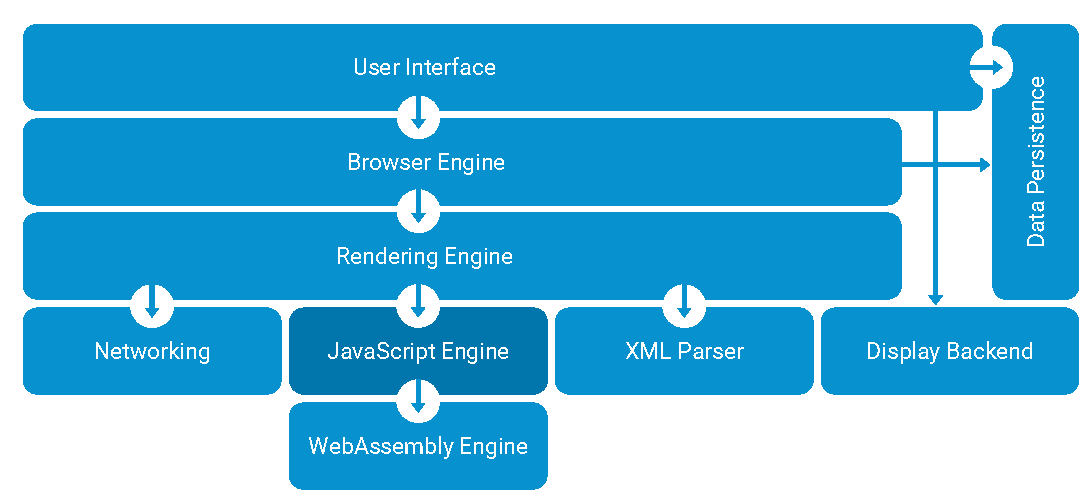
\includegraphics[width=16cm,keepaspectratio]{figures/reference-architecture}
\caption{Web browser reference architecture. Adapted from \textcite{GrosskurthGodfrey2005}.}
\label{reference-architecture}
\end{figure}

The component in a web browser that is focused on JavaScript interpretation and execution is called a JavaScript engine \parencite{JeonChoi2012} The JavaScript engine is illustrated in Figure \ref{reference-architecture} as a part of the web browser reference architecture developed by \textcite{GrosskurthGodfrey2005}. The way JavaScript is executed is somewhat different in different web browsers but all share a similar approach. Figure \ref{javascript-optimization} illustrates three tiers of executing JavaScript. The first tier is concerned with interpreting the source code in realtime, translating that into an Abstract Syntax Tree (AST) and use that to generate bytecode that is then executed. Before browser vendors saw a competitive in having a really fast JavaScript engine the first tier was the only job of the JavaScript engine. In the second and third tier the result of the compilation is stored and executed again, the JIT compilation and the optimized JIT compilation is invoked based on how ''hot'' the code is \parencite{KedlayaRobatmiliHardekopf2015,ParkKimParkMoon2018}.

\begin{figure}[!h]
\centering

\includegraphics[width=16cm,keepaspectratio]{figures/javascript-optimization}
\caption{JavaScript execution tiers. Adapted from \textcite{ParkKimMoon2017,ZhuykovVardanyanMelnikBuchatskiySharygin2015}.}
\label{javascript-optimization}
\end{figure}        

As another way to try to optimize JavaScript \textcite{ParkJungMoon2015,ZhuykovVardanyanMelnikBuchatskiySharygin2015} and others are currently experimenting with AOT compilation where JavaScript is actually compiled ahead of time instead of in realtime.

\subsubsection{TypeScript}

JavaScript does not have a static type system \parencite{Park2014}. TypeScript is a superset of JavaScript that adds type information \parencite{DeWolffHage2017}. Type information allows the programmer to see mistakes sooner during the development phase rather than later in runtime. In Listing \ref{listing:typescript} the JavaScript function \texttt{isPrime} has been enhanced with type information.

\lstinputlisting[label=listing:typescript,language=JavaScript,caption=prime.ts]{listings/isprime.ts}

Before TypeScript is published as part of a web site it is transformed to regular JavaScript using the TypeScript compiler \parencite{ReiserBlaser2017}. This does thus not directly solve the problem of performance, but decreases the number of runtime errors, and enables future backend optimizations such as improved guesses by the JIT-compiler.

\subsubsection{asm.js}

Another approach to optimize JavaScript is asm.js which is a subset of JavaScript focused on performance \parencite{Zakai2018}. If the browser understands asm.js it will skip certain steps in the JavaScript engine designed to optimize ''normal'' JavaScript, as it knows that asm.js is already optimized in certain ways. \textcite{Zakai2018} describes the idea behind asm.js as removing the dynamic and complex parts of JavaScript and thus ending up with a subset that is more easily optimized by the JavaScript engines.

\lstinputlisting[label=asmjs,language=JavaScript,caption=asm.js]{listings/asm.js}

Listing \ref{asmjs} shows an implementation of a string calculation length function written in asm.js containing two prominent differences between asm.js and regular JavaScript. On line 2, 6, and 8 a bitwise operator \texttt{|0} is used. The operator has no effect on the value of the result but provides a hint to the JavaScript engine that the result is of the type signed integer which is information that can be used by the JavaScript engine to optimize the performance \parencite{Zakai2018}. The use of \texttt{MEM8[]} on line 5 is another way to increase the performance in asm.js. In asm.js much of the memory is written to and read from a type buffer instead of relying on the slower garbage collector provided by the JavaScript engine \parencite{Zakai2011}.

Asm.js is not meant to be written by hand but rather serve as compilation target \parencite{VanEsNicolayStievenartDHondtDeRoover2016}. The tool Emscripten \parencite{Zakai2011} was so that source code written in languages such as C/C++ could be compiled to asm.js. As asm.js is a subset of JavaScript all browsers that can run JavaScript can run asm.js code that has been created by the Emscripten tool \parencite{HaasRossbergSchuffTitzerHolmanGohmanWagnerZakaiBastien2017}. Given this, it is not far fetched to call asm.js the assembly language of the web. However, asm.js \emph{is} JavaScript and JavaScript was never designed as a compilation target \parencite{Watt2018}.

\subsection{WebAssembly}

WebAssembly\footnote{\url{https://webassembly.org/}} (Wasm) is described by \textcite{Watt2018,JangdaPowersGuhaBerger2019} as a low-level language designed to become a universal compilation target for the web. According to the original authors \textcite{HaasRossbergSchuffTitzerHolmanGohmanWagnerZakaiBastien2017} it is a portable assembly-language for web browsers and future adaptations. Technically WebAssembly is bytecode created by \emph{compiling} (any form of) code to WebAssembly \parencite{Watt2018} which then can be executed in any WebAssembly-engine. This can be compared with JavaScript-code that is \emph{interpreted} while running inside a JavaScript-engine.

WebAssembly can be seen as a successor to earlier technologies such as asm.js from Mozilla (previously discussed) and Native Client (NaCL) from Google. NaCL executes native code in a separate part of Chrome and asm.js  \parencite{Zakai2018} is a subset of JavaScript optimized for performance \parencite{VanEsNicolayStievenartDHondtDeRoover2016} and can be interpreted in any web browser. Emscripten \parencite{Zakai2011}, a compiler based on LLVM \parencite{LattnerAdve2014} that originates as a source-to-source compiler from JavaScript to asm.js \parencite{Zakai2011} has been further developed \parencite{HaasRossbergSchuffTitzerHolmanGohmanWagnerZakaiBastien2017} and is now able to compile to both asm.js \emph{and} WebAssembly.

WebAssembly is the result of joint research and development between Apple, Google, Microsoft and Mozilla \parencite{HaasRossbergSchuffTitzerHolmanGohmanWagnerZakaiBastien2017}. WebAssembly has as the first technology since JavaScript full support in Chrome, Edge, Firefox and Safari and could as such be described as the forth core web technology (Figure \ref{webtechnologies-timeline}). Those web browsers that does not support WebAssembly can use asm.js as polyfill \parencite{HaasRossbergSchuffTitzerHolmanGohmanWagnerZakaiBastien2017}. WebAssembly is already being used where performance is of high importance, such as to generate cryptocurrency \parencite{RuthZimmermannWolsingHohlfeld2018}.

Initially WebAssembly supports code written in C/C++ \parencite{HaasRossbergSchuffTitzerHolmanGohmanWagnerZakaiBastien2017}. 
The focus on C/C++ is largely based on WebAssembly implementation limitations such as the lack of garbage collection. According to \textcite{HaasRossbergSchuffTitzerHolmanGohmanWagnerZakaiBastien2017} its a highly prioritized goal to allow WebAssembly to gain to access the web browsers built in garbage collector and that way support languages that use garbage collection.

WebAssembly is loaded as a module via a JavaScript API or another WebAssembly module \parencite{HaasRossbergSchuffTitzerHolmanGohmanWagnerZakaiBastien2017}. It is \emph{not} a goal to have WebAssembly replace JavaScript\footnote{\url{https://webassembly.org/docs/faq/\#is-webassembly-trying-to-replace-javascript}}, the idea is that they \emph{complement} each other. One example of how JavaScript and WebAssembly could complement each other is to port selected parts of a popular framework or web app for improved performance without changing the interface.

